%%%%%%%%%%%%%%%%%%%%%%%%%%%%%%%%%%%%%%%%%%%%%%%%%%%%%%%%
%%%%%%%%%%%%%%%%%%%%%%%%%%%%%%%%%%%%%%%%%%%%%%%%%%%%%%%%
\section{Miscellaneous}
\label{additional:misc}

%%%%%%%%%%%%%%%%%%%%%%%%%%%%%%%%%%%%%%%%%%%%%%%%%%%%%%%%
\subsection{Checking \texorpdfstring{$m$}{m} for the Model}
\label{additional:misc:enough_data}
% TODO
% TODO ref in text \cref{fig:additional:misc:enough_data}

\begin{figure}
\centering
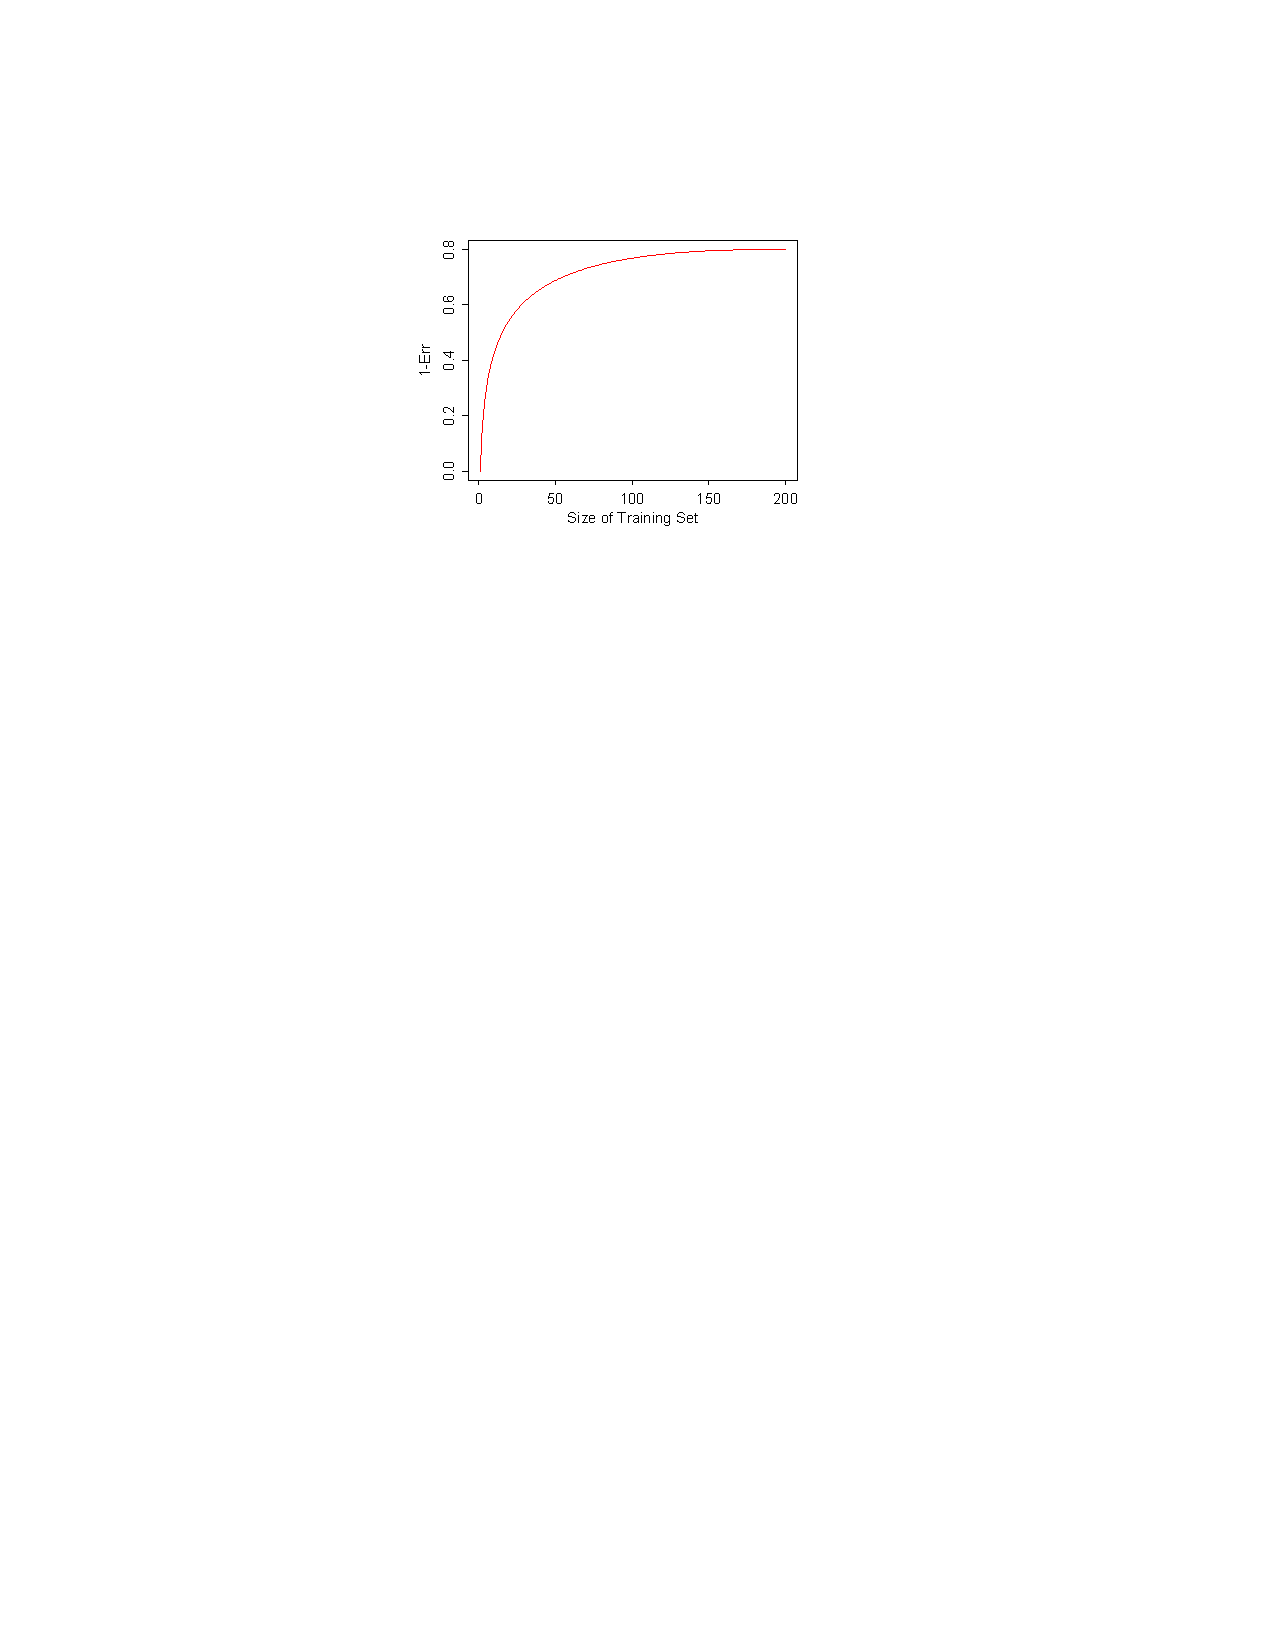
\includegraphics[width=0.8\textwidth]{figures/ml/acc_vs_m}
\caption{
Illustration of the decrease in classification error rate
with larger sets of training data \cite{HastieTF09}.
By artificially limiting the available number of data points $m$,
one can create a similar curve to verify that
there is enough statistics in the training data
for the complexity of the model under consideration.
Ideally the curve should reach a clear asymptote before the maximum $m$ is used.
}
\label{fig:additional:misc:enough_data}
\end{figure}

%%%%%%%%%%%%%%%%%%%%%%%%%%%%%%%%%%%%%%%%%%%%%%%%%%%%%%%%
\subsection{Factor Analysis}
\label{additional:misc:factor_ana}
% TODO

%%%%%%%%%%%%%%%%%%%%%%%%%%%%%%%%%%%%%%%%%%%%%%%%%%%%%%%%
\subsection{Optimization and Lagrange Multipliers}
\label{additional:misc:opt}
% TODO

%%%%%%%%%%%%%%%%%%%%%%%%%%%%%%%%%%%%%%%%%%%%%%%%%%%%%%%%
\subsection{Information Theory}
\label{additional:misc:info_theory}
% TODO
% TODO Entropy, significance of bits

%%%%%%%%%%%%%%%%%%%%%%%%%%%%%%%%%%%%%%%%%%%%%%%%%%%%%%%%
\subsection{Modulo Operations}
\label{additional:misc:modulo}

\begin{subequations}\label{eq:additional:misc:modulo}
\begin{align}
\left(A~\text{mod}~C\right)~\text{mod}~C &= A~\text{mod}~C, \label{eq:misc:additional:modulo:basic} \\
\left(A \pm B\right)~\text{mod}~C &= \left(A~\text{mod}~C \pm B~\text{mod}~C\right)~\text{mod}~C, \label{eq:misc:additional:modulo:pm} \\
\left(A \times B\right)~\text{mod}~C &= \left(A~\text{mod}~C \times B~\text{mod}~C\right)~\text{mod}~C, \label{eq:misc:additional:modulo:multiplication} \\
A^{B}~\text{mod}~C &= \left(\left(A~\text{mod}~C\right)^{B}\right)~\text{mod}~C. \label{eq:misc:additional:modulo:exp}
\end{align}
\end{subequations}

%%%%%%%%%%%%%%%%%%%%%%%%%%%%%%%%%%%%%%%%%%%%%%%%%%%%%%%%
\subsection{Mathematical Relations}
\label{additional:misc:math}

\begin{subequations}\label{eq:additional:misc:math}
\begin{align}
e^{x} &= \sum_{k=0}^{\infty} \frac{x^{k}}{k!} \label{eq:additional:misc:math:ex} \\
e^{x} &= \lim_{n \to \infty} \left(1 + \frac{x}{n}\right)^{n} \label{eq:additional:misc:math:ex_limit} \\
\frac{1}{1-r} &= \sum_{k=0}^{\infty} r^{k}, \quad \abs{r} < 1 \label{eq:additional:misc:math:geometric} \\
e^{-i x} &= \cos\left(x\right) + i \sin\left(x\right) \label{eq:additional:misc:math:eulers_formula} \\
2 \cos\left(x\right) &= e^{i x} + e^{-i x} \label{eq:additional:misc:math:cos_exp} \\
2i \sin\left(x\right) &= e^{i x} - e^{-i x} \label{eq:additional:misc:math:sin_exp} \\
\abs{\mathbf{u} + \mathbf{v}} &\leq \abs{\mathbf{u}} + \abs{\mathbf{v}} \label{eq:additional:misc:math:triangle_inequality} \\
\abs{\braket{u}{v}}^{2} &\leq \braket{u} \braket{v} \label{eq:additional:misc:math:cauchy_schwarz_inequality} \\
n^{k} &= N\left(\text{Permutations Length, $k$ with Repetition}\right) \label{eq:additional:misc:math:permutations_with_repetition} \\
\frac{n!}{\left(n-k\right)!} &= N\left(\text{Permutations Length $k$, without Repetition}\right) \label{eq:additional:misc:math:permutations_without_repetition} \\
\frac{n!}{k!\left(n-k\right)!} &= {n \choose k} = N\left(\text{Combinations of Length $k$ from $n$}\right) \label{eq:additional:misc:math:binomial_coefficient} \\
\overline{A \cap B} &= \overline{A} \cup \overline{B},\quad \overline{A \cup B} = \overline{A} \cap \overline{B} \label{eq:additional:misc:math:de_morgan} \\
\dv{}{x}\, a^{x} &= a^{x} \ln\left(a\right), \quad 0 < a \label{eq:additional:misc:math:diff_exp_gen} \\
\dv{}{x}\, \log_{a}\left(x\right) &= \frac{1}{x \ln a} \label{eq:additional:misc:math:diff_log_gen}
\end{align}
\end{subequations}
